\RequirePackage[2020-02-02]{latexrelease}
\documentclass[letter,scriptaddress,twocolumn, prl]{revtex4}

\usepackage{amsmath}%,amssymb} 
\usepackage{makeidx}
\usepackage{amsfonts}
\usepackage[ansinew]{inputenc}
%\usepackage[usenames,dvipsnames]{pstricks}
%\usepackage{subfigure}
\usepackage{epsfig}
\usepackage{float}
%\usepackage{pst-grad} % For gradients
%\usepackage{pst-plot} % For axes
\usepackage[colorlinks,hyperindex]{hyperref}
\hypersetup
{
colorlinks,%
citecolor=black,%
linkcolor=black,%
urlcolor=black,%
}

\setlength\textheight{24.5cm}

% --- Comandos novos ---
\newcommand{\dket}[1]{\left| #1 \right)}
\newcommand{\E}[1]{\frac{\hbar^2 #1 ^2}{2m_0}}
\newcommand{\dbra}[1]{\left( #1 \right|}
\newcommand{\dsubmin}[1]{\left( #1 \right)}
\newcommand{\dbraket}[2]{\left( #1 | #2 \right)}
\newcommand{\dbraketm}[3]{\left( #1 \left| #2 \right| #3 \right)}
\newcommand{\ket}[1]{\left| #1 \right\rangle}
\newcommand{\bra}[1]{\left\langle #1 \right|}
\newcommand{\submin}[1]{\left\langle #1 \right\rangle}
\newcommand{\braket}[2]{\left\langle #1 \right. \left| #2 \right\rangle}
\newcommand{\braketm}[3]{\langle #1 \mid #2 \mid #3 \rangle}
\newcommand{\pinterno}[2]{\left( #1 , #2 \right)}
\newcommand{\comut}[2]{\left[ #1 , #2 \right]} % THE COMUTATOR
\newcommand{\seitz}[2]{\left\{ \, #1 \mid  #2 \, \right\}}
\newcommand{\rep}{\emph{rep} }
\newcommand{\irep}{\emph{irrep} }
\newcommand{\ordem}[1]{\mid #1 \mid}
\newcommand{\op}[1]{\mathbb #1 }
\newcommand{\group}[1]{\mathcal #1 }
\newcommand{\vet}[1]{\mathbf #1 }
\newcommand{\argu}[1]{\left( #1 \right)}
\newcommand{\kp}{\vet{k}\cdot\vet{p}}

\makeindex

%--------------------------------------------------------
\begin{document}

\title{Computational Simulation of the 2d Ising Model}

\author{Alex Roseman}
\author{Adrian Hall}
\date{\today}

\begin{abstract}

\end{abstract}

\maketitle

\begin{figure*}[t]
	\begin{center}
		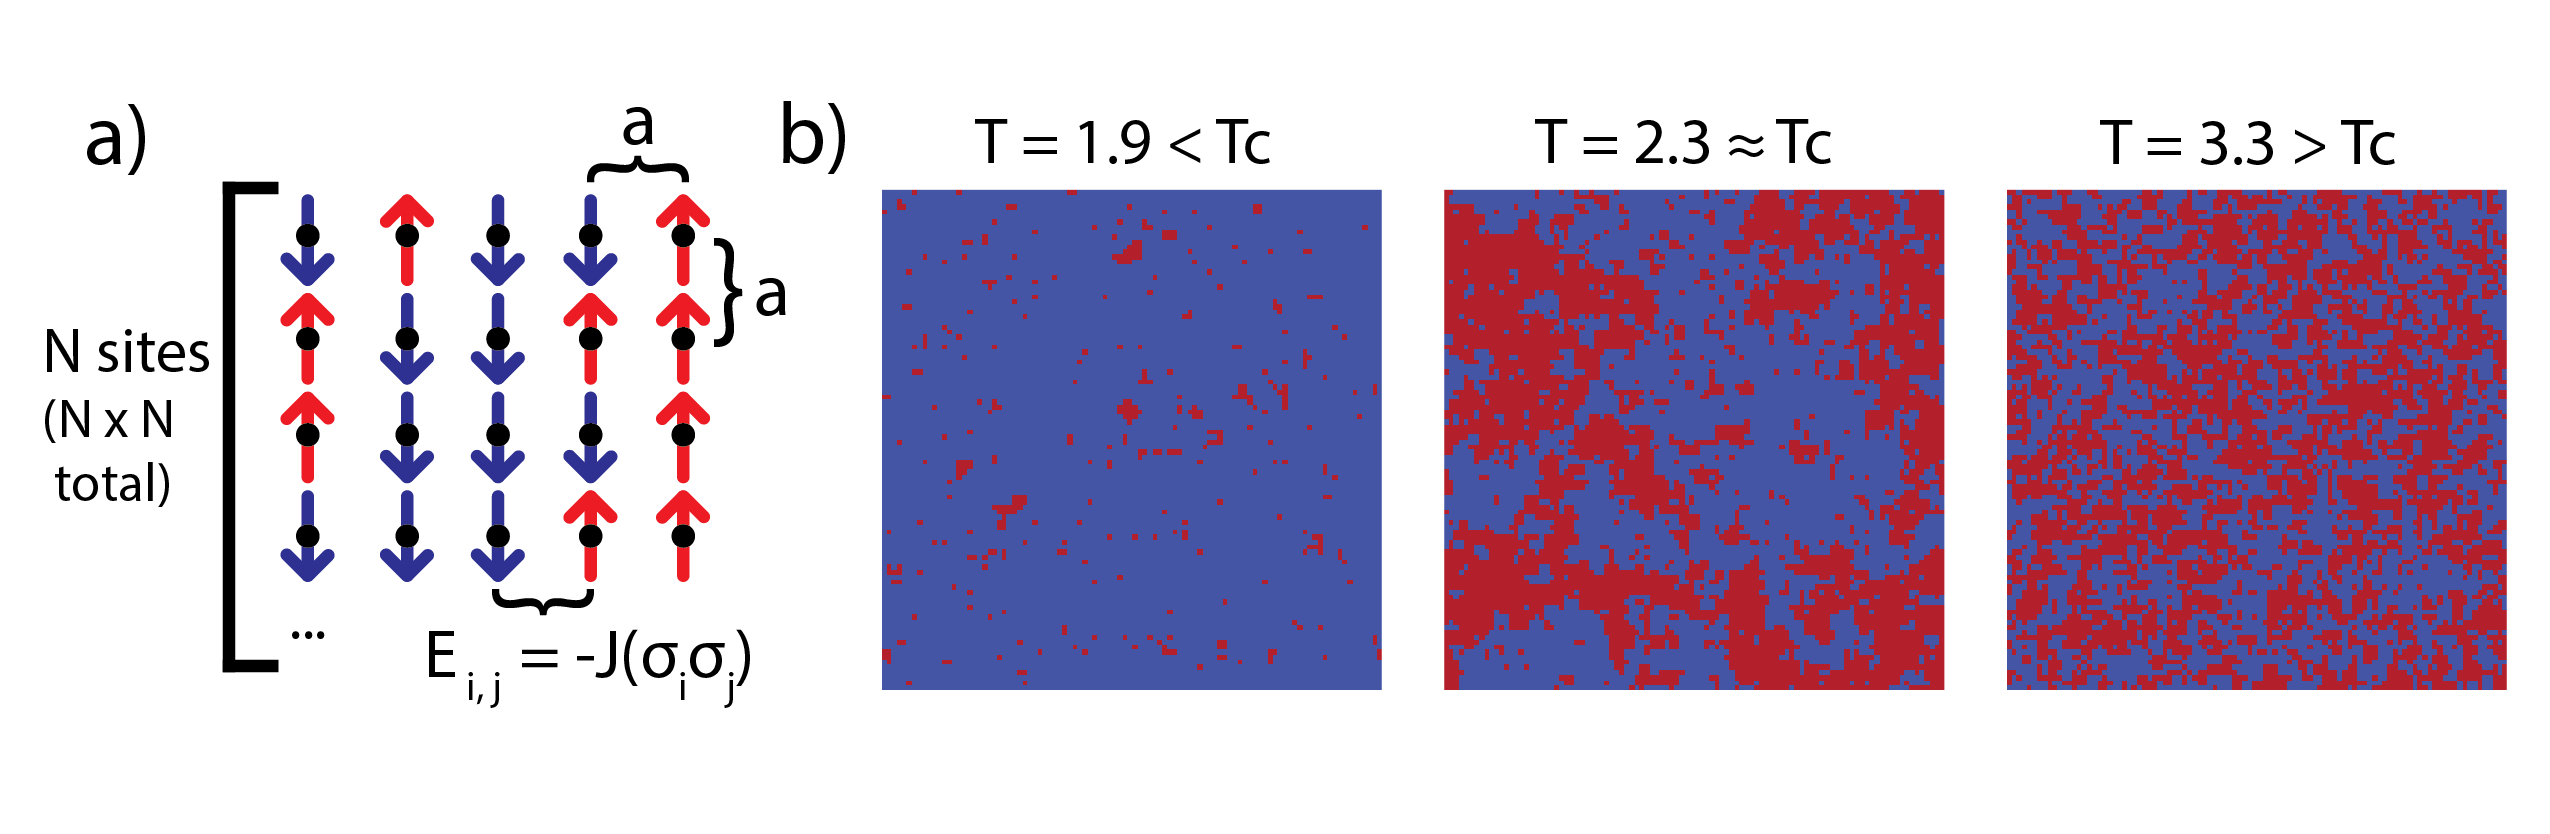
\includegraphics[width=1\textwidth]{figs/fig1.png}
		\caption{a. diagram of the lattice. We use N=100 throughout. $E_{i, j}$ is neighbor spin interaction - adjacents only, wraps (each site has 4 neighbors). "a" is lattice distance (1), J = 1, spin = $\pm 1$. b. Snapshots after ~10 million simulation steps at the given temperature, showing typical states below, near, and above Tc. Red is spin up, blue spin down.}
		\label{fig:fig1}
	\end{center}
\end{figure*}

\section{Introduction}

\begin{equation}
	\label{eq:hamiltonian}
	H = -J \sum_{\left\langle i, j \right\rangle}\sigma_i\sigma_j - B \sum_i\sigma_i
\end{equation}

\begin{equation}
	\label{eq:Tc}
	T_c = \frac{2}{\ln{(1+\sqrt{2})}} \approx 2.269 (J/k_B)
\end{equation}

\section{Methods}

\section{Data and Analysis}

\begin{figure}[h]
	\begin{center}
		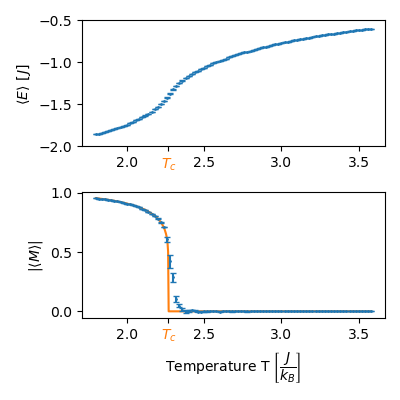
\includegraphics[width=.5\textwidth]{figs/fig2_EMplots.png}
		\caption{Mean energy (top) and absolute magnetization (bottom) per lattice site as computed by MCMC simulation at a range of temperatures. Data is drawn from 97 independent simulations: each data point is the average value of $\left\langle M \right\rangle$ over all simulations; each standard error is the standard error of the mean of $\left\langle M \right\rangle$ over all simulations, treating each $\left\langle M \right\rangle$ as an independent measurement. Analytic Tc (red) and analytic curves (green) plotted for comparison. At first glance, our system appears to reach phase transition at lower temperature than the analytic $T_c$.}
		\label{fig:fig2}
	\end{center}
\end{figure}



\begin{figure}[h]
	\begin{center}
		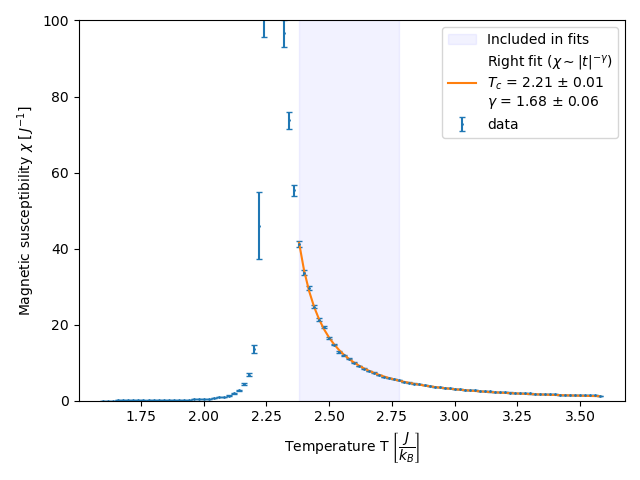
\includegraphics[width=.4\textwidth]{figs/fig3_chi.png}
		\caption{Magnetic susceptibility at a range of temperatures. Susceptibility is calculated from variance in M over each simulation, which is taken as a single measurement. Data points on this graph are the mean of variance(M) over all 97 simulations at a given temperature, and error bars on this graph are the standard error of this mean. Shown in orange is a power law fit with $T_c$ and $\gamma$ considered as free variables, using only the data in the shaded column. NOTE: we intend to merge figures 3 and 4 into a single figure with 2 graphs.}
		\label{fig:fig3a}
	\end{center}
\end{figure}
\begin{figure}[h]
	\begin{center}
		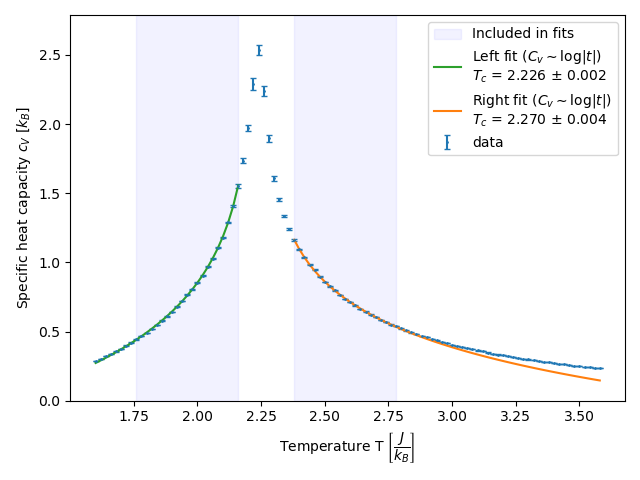
\includegraphics[width=.4\textwidth]{figs/fig3_cv.png}
		\caption{Specific heat at a range of temperatures. Like susceptibility, specific heat is calculated from variance in E across MCMC steps. Data points on this graph are the mean of variance(E) over all 97 independent simulations at a given temperature, and error bars on this graph are the standard error of this mean. Shown in orange and green are logarithmic fits in which $T_c$ was considered a free variable, using only the data in the shaded columns. We generated separate fits on the left and right of Tc. Although the power law should be symmetric, we find significantly different results for Tc. NOTE: we intend to merge figures 3 and 4 into a single figure with 2 graphs.}
		\label{fig:fig3b}
	\end{center}
\end{figure}
\begin{figure}[h]
	\begin{center}
		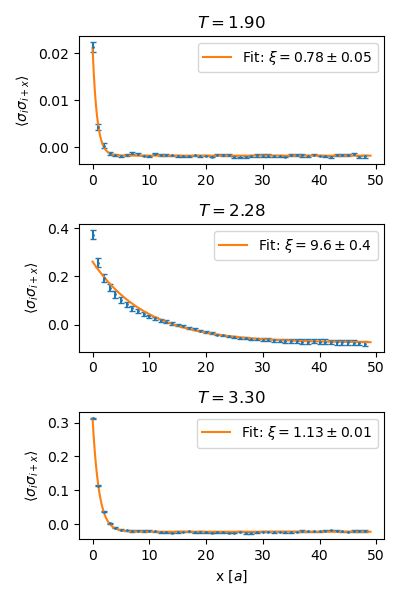
\includegraphics[width=.4\textwidth]{figs/fig4_autocors.png}
		\caption{Autocorrelation functions at representative temperatures: below, near, and above $T_c$. Shown in orange are exponential decay functions fit by least-squares regression to the positive portion of the autocorrelation data, with length scale parameter $\xi$. Autocorrelation seems to become negative (i.e. anticorrelated) after sufficient lattice distance, leading the exponential fit to deviate significantly from the data. This likely plays a role in our terrible estimate for $\nu$. Note: we intend to merge Figs. 5 and 6.}
		\label{fig:fig4a}
	\end{center}
\end{figure}
\begin{figure}[h]
	\begin{center}
		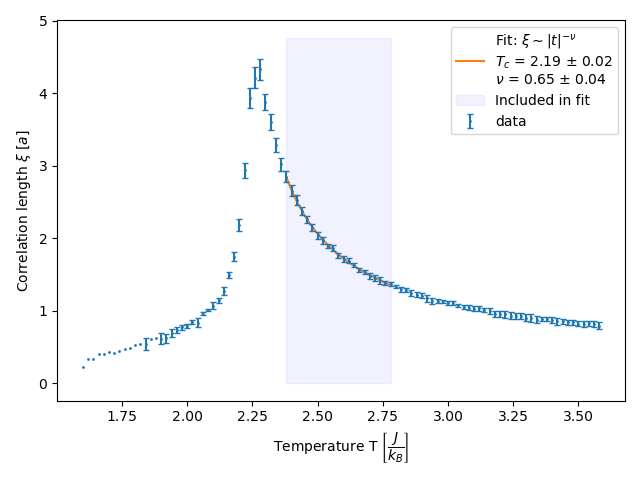
\includegraphics[width=.4\textwidth]{figs/fig4_xi.png}
		\caption{Correlation length $\xi$ at a range of temperatures. These data points are drawn from the fits depicted in Fig. 5, with all the inaccuracy that entails. Uncertainties are drawn from Scipy's curve fit covariance matrix. We intend to include a complete description of the nature of these uncertainties in the body of our report. As with $\chi$ and $c_v$, we fit a power law function (orange) to the data in the shaded region, with $T_c$ and $\nu$ as free parameters. Note: we intend to merge Figs. 5 and 6.}
		\label{fig:fig4b}
	\end{center}
\end{figure}
\begin{figure*}[h]
	\begin{center}
		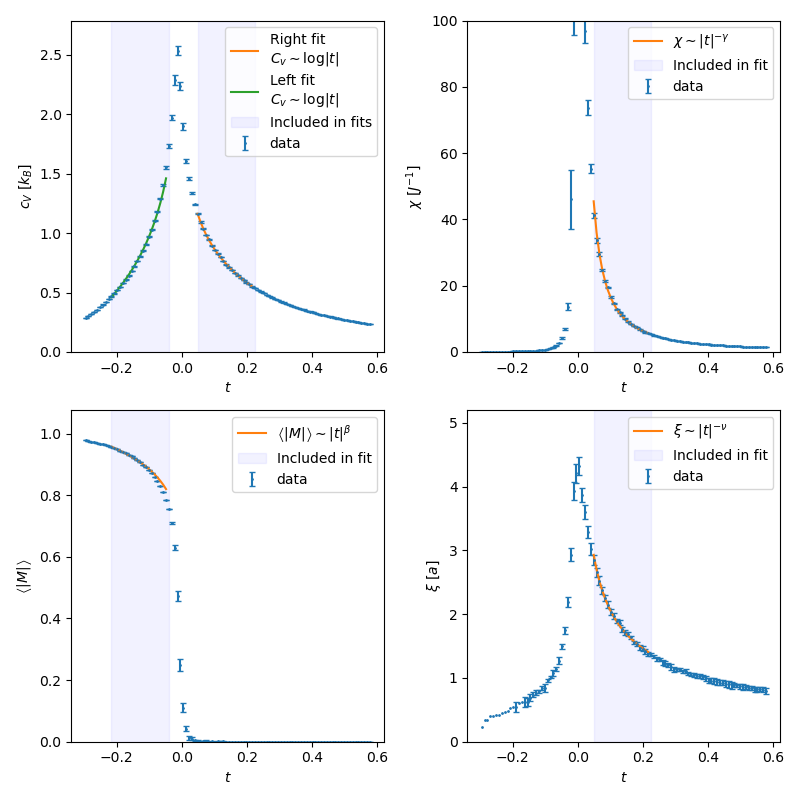
\includegraphics[width=1\textwidth]{figs/fig5_crit_exponents.png}
		\caption{Power law fits for the critical exponents for $c_V$ ($\alpha$) (upper left), $\chi$ ($\gamma$) (upper right), $|M|$ ($\beta$) (lower left), and $\xi$ ($\nu$) (lower right). We attempt to show $\alpha = 0$ by successfully fitting a logarithmic function to $c_V$. In each graph, the x-axis is the normalized temperature $t = \frac{T - T_c}{T_c}$, where $T_c$ is the analytic value of $T_c$. As before, only data from the shaded regions was used for fits. We find the following values: $\gamma = 1.40 \pm .01$, $\beta = 0.103 \pm .002$, $\nu = 0.49 \pm .01$. All critical exponents are, of course, unitless. We have not checked identities because these values are clearly broken, $\nu$ especially (see abstract for details).}
		\label{fig:fig5}
	\end{center}
\end{figure*}

\section{Acknowledgements}
	Prof. Navon, Prof. Newburgh, HongJoon

\bibliographystyle{unsrt} 
%\bibliography{/home/thiago/bibtex/articles,/home/thiago/bibtex/books}

\begin{thebibliography}{}
	
	\bibitem{Onsager}
	Lars Onsager,
	\textit{Crystal Statistics. I. A Two-Dimensional Model with an Order-Disorder Transition},
	Physical Review {\bf 65}, 117 (1944).
	
	
\end{thebibliography}

\appendix
\section{\\Appendix A: Convergence}

\begin{figure}[h]
	\begin{center}
		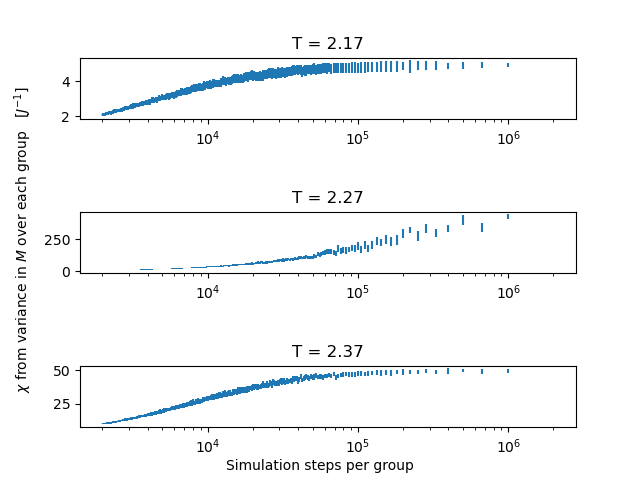
\includegraphics[width=.4\textwidth]{figs/figA1.png}
		\caption{$\chi$ values calculated with data from a simulation of 2,000,000 analyze steps. The total 2,000,000 steps were split as evenly as possible into groups of $n_{steps}$ (x axis), and variance in M was calculated across each group. Each data point is the average variance over all such groups.}
		\label{fig:figA1}
	\end{center}
\end{figure}

\end{document}
